% !TeX root = master.tex
\documentclass[12pt]{article}
 
\usepackage[margin=1in]{geometry} 
\usepackage{amsmath,amsthm,amssymb}
\usepackage[spanish]{babel}
\usepackage[utf8]{inputenc}
\usepackage{tikz-cd}
\usepackage{amsmath}
\usepackage[shortlabels]{enumitem}
\usepackage{mathtools}

% cosas entre comillas 
\usepackage{csquotes}

\usepackage{tikz}


\usepackage{xcolor}

\usepackage{config}

\newtheorem{theorem}{Teorema}[section]
\newtheorem{lemma}[theorem]{Lema}
\newtheorem{prop}[theorem]{Proposición}
\newtheorem{coro}[theorem]{Corolario}
\newtheorem{conj}[theorem]{Conjetura}
\newtheorem{ejercicio}{Ejercicio}[section]
\newtheorem*{ejercicio*}{Ejercicio}
\theoremstyle{definition}
\newtheorem{definition}[theorem]{Definición}
\newtheorem{example}[theorem]{Ejemplo}
\theoremstyle{remark}
\newtheorem{remark}[theorem]{Nota}
\newtheorem{notacion}[theorem]{Notación}
\newcommand{\continuas}[1][]{C^{ #1 }[a,b]}
\newcommand{\continuasabierto}[1][]{C^{ #1 }(a,b)}
\newcommand{\soportecompacto}{\mathcal{D}(a,b)}
\newcommand{\xcero}{(a,b)}
\newcommand{\xcerocerrado}{[a,b]}
\newcommand{\fvariaciones}{F(x,y(x),y'(x))}

\begin{document}

\title{Modelos Matemáticos II}
\author{Antonio Gámiz Delgado\\ Universidad de Granada} 
 
\maketitle

\chapter{Cálculo de variaciones}

\section{Herramientas previas y repaso}

Necesitaremos recordar algunas nociones y teoremas básicos sobre derivabilidad:

\begin{theorem}[derivada de una integral respecto de un parámetro]
\label{derivadaparametro}
Sea $X\subset\R^n$ y $(X,\mathcal{A},\mu)$ un espacio medible, $I$ un intervalo cerrado y sea $\funcion{f}{I\times X}{\R}$ tal que:

\begin{enumerate}[(a)]
\item $\forall t \in I$, $x\mapsto f(t,x)$ es integrable.
\item $\forall x\in X$, la función $t\mapsto f(t,x)$ es derivable en $t\in I$.
\item Existe $\funcion{g}{X}{\R}$ integrable tal que
\[
\left|\derivada{f}{t}(t,x)\right|\leq |g(x)| \espacio \forall x\in X\; \forall t \in I
\]
Entonces la función $F(t)=\int_Xf(t,x)dx$ es derivable en $t_0$ y la derivada es 
\[
F'(t_0)=\displaystyle\int_X\derivada{f}{t}(t_0,x)dx
\]
\end{enumerate}

\end{theorem}

TODO: añadir resto de resultados usados de otras asignaturas que no recordábamos

\section{Problema general del cálculo de variaciones}

Primeramente definimos un tipo de funciones llamadas \textit{funciones test} o \textit{funciones de la clase de Schwartz}, junto con algunos resultados que usaremos bastante para trabajar con ellas.

\begin{definition}
\label{funcionestest}
Dado $I$ intervalo, se llama \textit{espacio de funciones test} al conjunto:
\[
\mathcal{D} = \mathcal{D}(a,b) = \{\phi\in C^{\infty}(a,b): \; \exists J\subset(a,b) \text{ compacto: } \phi(x)=0 \text{ si } x \notin J\}
\]
\end{definition}

\begin{lemma}
\label{existenciaphi}
Dado $x_0\in(a,b)$ y $\varepsilon>0$ tal que $[x_0-\varepsilon, x_0+\varepsilon]\subset(a,b)$, existe $\phi\in\mathcal{D}(a,b)$ tal que $\phi(x)>0$ si $x\in(x_0-\varepsilon,x_0+\varepsilon)$ y $\phi(x)=0$ en otro caso.
\end{lemma}

\begin{proof}
La demostración la vamos a hacer por construcción. Sea $\funcion{g}{\R}{\R}$ definida por:
\[
g(x)=\left\{
\begin{array}{cc}
e^{1/x} & x<0 \\
0 & x\geq 0
\end{array}
\right.
\]
Tenemos que $\limite{x}{0^-}{g(x)}=0$, luego $g$ es continua. Veamos que de hecho $g\in C^{\infty}$. Su derivada es:
\[
g'(x)=\left\{
\begin{array}{cc}
e^{1/x}\left(-\frac{1}{x^2}\right) & x<0 \\
0 & x> 0
\end{array}
\right.
\]
Mediante un proceso iterativo llegamos a:
\[
g^{n)}(x)=\left\{
\begin{array}{cc}
e^{1/x}\frac{R(x)}{x^{2n}} & x<0 \\
0 & x> 0
\end{array}
\right.
\]
donde $R(x)$ es un cierto polinomio que no nos interesa calcular. Queremos ver que 
\[\limite{x}{0^-}{g^{n)}(x)}=0,\]
con lo cual, $g\in C^n$. Haciendo el cambio $y=-\frac{1}{x}$, el anterior límite equivale a 
\[
\limite{y}{+\infty}{\frac{y^{2n}}{e^y}}=0 \Rightarrow g\in C^{n} \;\forall n \in\N \Rightarrow g\in C^{\infty}
\]
Con lo anterior, solo nos queda definir la función buscada de forma que sea una función test, es decir, la definimos como:
\[
\phi(x)=g(x-(x_0+\varepsilon))g((x_0-\varepsilon)-x) \espacio \varepsilon>0 
\]

\end{proof}


\begin{theorem}
\label{theorem:1.3}
Sea $f\in \continuas$ tal que
\[
\int f(x)\phi(x)dx=0 \hspace{1cm} \forall \phi \in \soportecompacto
\]
Entonces $f(x)=0 \;$  $\forall x\in [a,b]$.
\end{theorem}

\begin{proof}
Sea $\bar{x}\in \xcero$ y supongamos por reducción al absurdo que $f(\bar{x})\neq 0$. Podemos suponer $f(\bar{x})>0$. Aplicando el teorema de conservación del signo, obtenemos $\varepsilon>0$ tal que $f(x)>0 \text{ si } x \in (\bar{x}-\varepsilon,\bar{x}+\varepsilon)$.

Por el lema \ref{existenciaphi}, existe una función test $\phi$ tal que $\phi(x)>0$ si $x\in(\bar{x}-\varepsilon, \bar{x}+\varepsilon)$ y $0$ en otro caso. Luego:
\[
0=\int_{a}^{b}f(x)\phi(x)dx=\int_{\bar{x}-\varepsilon}^{\bar{x}+\varepsilon}f(x)\phi(x)dx>0 \Rightarrow f(\bar{x})=0
\]
Como $\bar{x}$ era arbitrario, tenemos que $f(\bar{x})=0 \; \forall \bar{x}\in\xcero$, y por la continuidad de $f$ podemos extenderlo a los extremos también, es decir, $f(a)=f(b)=0$.

\end{proof}

\subsection{Cálculo de extremales}

Sea $\Omega\subset\R^3$, definamos $F:\Omega \longrightarrow \R$ tal que $(x,y,p)\longmapsto F(x,y,p)$. Supongamos que $F\in C^1(\Omega)$  respecto de las dos últimas variables, es decir, existen $\derivada{F}{y}$ y $\derivada{F}{p}$, continuas. 

Usando la función anterior, podemos definir el siguiente funcional:

\begin{equation}\label{funcional}
L(y) = \int_{a}^{b}\fvariaciones dx 
\end{equation}


Nuestro objetivo en este apartado será encontrar \textit{extremales} de ese funcional, es decir, máximos o mínimos.

\begin{notacion}
Normalmente, a las derivadas parciales las denotaremos por:
\[
\derivada{F}{x}=F_x
\]
\end{notacion}

Los \textit{extremales} los buscaremos entre los elementos de un conjunto de funciones cumpliendo ciertas propiedades:

\begin{definition}
\label{espaciofuncionesbuenas}

Sea $\Omega\subset\R^3$ y $F:\Omega\longrightarrow \R$ funcional en las condiciones anteriores. Definimos entonces el siguiente conjunto:

\begin{equation}\label{espaciofunciones}
D=\{y\in\continuasabierto\cap\continuas[1]: \text{ se cumplen (a),(b) y (c)}\}
\end{equation}

\begin{enumerate}[(a)]
\item $(x,y(x),y'(x))\in\Omega \espacio \forall x\in\xcero$
\item $y(a)=y_0$ e $y(b)=y_1$ (\textit{Condición de contorno})
\item $\displaystyle\int_{a}^b\Big|\fvariaciones\Big|dx<+\infty$ 
\end{enumerate}

\end{definition}

El siguiente teorema nos proporcionará una condición sobre las derivadas parciales de $F$, que nos ayudará a buscar \textit{extremales}. Para su demostración necesitaremos el siguiente lema:

\begin{lemma}
\label{lemmatecnico}
Sea $\{s_n\}\longrightarrow 0$ una sucesión de números reales y $\phi\in \soportecompacto$, existe $n_0\in\N$ tal que si $y\in D$, entonces $y+s_n\phi\in D \espacio \forall n\geq n_0$.
\end{lemma}
\begin{proof}

Sea $\phi\in\soportecompacto$ y $K=\supp\phi$.Tenemos que comprobar que $y+s_n\phi$ cumple las condiciones de la definición \ref{espaciofuncionesbuenas}.

\begin{enumerate}[(a)]
\item Razonemos por reducción al absurdo. Supongamos que hay infinitos valores de $n\in\mathbb{N}$ tales que $(x_n,y(x_n)+s_n\phi(x_n),y'(x_n)+s_n\phi'(x_n))\notin \Omega$ para algún $x_n\in(a,b)$. Tomando una parcial si es necesario, podemos suponer una sucesión $\{x_n\}$ tal que para cada $n\in\mathbb{N}$, $(x_n,y(x_n)+s_n\phi(x_n),y'(x_n)+s_n\phi'(x_n))\notin \Omega \Rightarrow x_n\in\supp\phi$, ya que si no estuviera, tendríamos que $\phi(x_n)=0$ y $(x_n,y(x_n),y'(x_n))\in \Omega$. Como el soporte es compacto, podemos suponer que $\{x_n\}\longrightarrow\bar{x}\in\supp\phi\in(a,b)$. Si tomamos límite:
\[
\limitemasinfinito{n}{(x_n,y(x_n)+s_n\phi(x_n),y'(x_n)+s_n\phi'(x_n))}=(\bar{x},y(\bar{x}),y'(\bar{x}))\notin\Omega 
\]
porque el complementario de $\Omega$ es cerrado y el límite se queda fuera, llegando así a un absurdo. Por tanto, debe existir un $n_0\in\mathbb{N}$ tal que $(x_n,y(x_n)+s_n\phi(x_n),y'(x_n)+s_n\phi'(x_n))\in \Omega\quad\forall n\geq n_0$.
\item Evidente, ya que $\phi(a)=\phi(b)=0$.
\item Tomando $n\geq n_0$,de (a) tenemos:
\[
\integral{a}{b}{\Big|F(x,y(x)+s_n\phi(x),y'(x)+s_n\phi'(x))\Big|dx}=\]
\[
=\integral{(a,b)\backslash K}{}{\Big|F(...)\Big|dx}+\integral{K}{}{\Big|F(...)\Big|dx} < +\infty
\]
El primer término es finito ya que, fuera de $K$, $\phi=0$, luego ese término coincide con $\integral{(a,b)\backslash K}{}{\Big|F(x,y(x),y'(x))\Big|dx}$, que
es finito porque $y\in D$.
El segundo término lo es porque ser la integal de una función continua en un compacto. 
\end{enumerate}
\end{proof}
Lo que nos asegura este lema es que podamos sumar una perturbación \textit{pequeña} a nuestro extremal sin \textit{salirnos} de $D$.

\begin{theorem}
\label{theorem:1.7}
Si $\bar{y}\in D$ es un extremal, entonces:
\[
\integral{a}{b}{F_y(x,\bar{y}(x), \bar{y}'(x))}\phi(x)dx+\integral{a}{b}{F_p(x,\bar{y}(x), \bar{y}'(x))}\phi'(x)dx=0 \espacio \forall \phi\in \soportecompacto
\]
A $\bar{y}$ se le suele llamar \textbf{función crítica}.
\end{theorem}

\begin{proof}
Sean $\bar{y}\in D$ extremal y $\phi\in\soportecompacto$. Definimos el funcional $g:\R\longrightarrow\R$ tal que $g(s)=L(\bar{y}+s\phi)$.

Por el lema anterior, existe $\varepsilon>0$ tal que $g$ está bien definida en $(-\varepsilon,\varepsilon)$.

Ahora queremos derivar $g$ respecto de $s$, pero necesitamos que esté definida en un intervalo cerrado (por el teorema \ref{derivadaparametro}). Para ello, tomamos un intervalo cerrado $J$ de forma que $\supp (\phi)\subset J\subset [a,b]$. 

Derivamos $g$ respecto de $s$:
\[
g'(s)=\left(
\integral{[a,b]}{}{F(x,\bar{y}+s\phi(x),\bar{y}'+s\phi'(x))dx}
\right)'=
\]
\[
=\left(
\integral{[a,b]\backslash J}{}{F(x,\bar{y}+s\phi(x),\bar{y}'+s\phi'(x))dx}+
\integral{J}{}{F(x,\bar{y}+s\phi(x),\bar{y}'+s\phi'(x))dx}
\right)'
\]
Usando que $\integral{[a,b]\backslash J}{}{F(x,\bar{y}+s\phi(x),\bar{y}'+s\phi'(x))dx}\phi(x)$ es una constante (por que $\bar{y}\in D$ y $\phi = 0$ en $[a,b]\backslash J$) cuya derivada es cero, obtenemos que:
\[
g'(s)= \integral{J}{}{\Big(F_y(x,\bar{y}+s\phi(x),\bar{y}'+s\phi'(x))\phi(x)+F_p(x,\bar{y}+s\phi(x),\bar{y}'+s\phi'(x))\phi'(x)\Big)dx}
\]
Como $\phi=0=\phi'$ fuera de $J$
\[
g'(s)= \integral{[a,b]}{}{\Big(F_y(x,\bar{y}+s\phi(x),\bar{y}'+s\phi'(x))\phi(x)+F_p(x,\bar{y}+s\phi(x),\bar{y}'+s\phi'(x))\phi'(x)\Big)dx}
\]
Si evaluamos ahora $g'$ en 0 y usamos que $\bar{y}$ es extremal, tenemos:
\[
g'(0)=\integral{a}{b}{\Big(F_y(x,\bar{y},\bar{y}')\phi+F_p(x,\bar{y},\bar{y}')\phi'\Big)dx}=0 
\]
\end{proof}

\subsection{Ecuación de Euler}

Usando el teorema anterior vamos a llegar a una ecuación diferencial de segundo orden que nos ayudará a resolver este problema. Definimos $Z(x)=F_p(x,y(x),y'(x))$, nuestro objetivo ahora es imponer condiciones suficientes para que $Z(x)\in C^1(a,b)$, para poder derivarla y obtener una ecuación diferencial en $y'$.

Para continuar necesitamos un lema previo:

\begin{lemma}
Sea $Z\in C^1(x_0,x_1)$, entonces:
\[
\integral{a}{b}{Z(x)\phi'(x)dx}=-\integral{a}{b}{Z'(x)\phi(x)dx} \espacio \forall \phi\in\soportecompacto
\]
\end{lemma}

\begin{proof}

Resolviendo la integal por partes tenemos:
\[
\left.\begin{array}{cc}
u=Z(x) & du=Z'(x)dx\\
dv=\phi'(x)dx & v=\phi
\end{array}\right\} \Rightarrow\integral{a}{b}{Z(x)\phi'(x)dx}=Z(x)\phi(x)\Big|_a^b-\integral{a}{b}{Z'(x)\phi(x)dx}=
\]
\[
=-\integral{a}{b}{Z'(x)\phi(x)dx}
\]

\end{proof}

Este lema nos permite \enquote{intercambiar la derivada de sitio}.
Usando ahora el Teorema \ref{theorem:1.7} (podemos usarlo porque $y$ es función crítica) y el lema anterior, tenemos:
\[
0=\integral{a}{b}{F_y(x,y, y')}\phi(x)dx+\integral{a}{b}{F_p(x,y,y')}\phi'(x)dx= 
\]
\[
=\integral{a}{b}{F_y(x,y, y')}\phi(x)dx+\integral{a}{b}{Z(x)}\phi'(x)dx=
\]
\[
=\integral{a}{b}{F_y(x,y, y')}\phi(x)dx-\integral{a}{b}{Z'(x)}\phi(x)dx=
\]
\[
=\integral{a}{b}{\Big(F_y(x,y, y')-Z'(x)\Big)}\phi(x)dx=0 \espacio \forall\phi\in\soportecompacto
\]
Y usando ahora el Teorema \ref{theorem:1.3} nos queda:
\[
F_y(x,y,y')-Z'(x)=0 \espacio \forall x \in\xcero
\]
Que denoteramos por:
\[
\frac{d}{dx}F_p-F_y(x,y,y')=0 \espacio \textbf{(Ecuación de Euler)}
\]
Las condiciones sobre $F$ se pueden rebajar con el siguiente teorema:

\begin{theorem} 
\label{theorem:12}
Si $F\in C^1_{yp}$, $y'\in C^1$, función crítica, entonces:
\[
Z(x)=F_p(x,y(x),y'(x))\in C^1
\]
\[
Z'(x)=F_y(x,y(x),y'(x))
\]
\end{theorem}

Ya tenemos la ecuación que queremos resolver. La demostración del teorema es consecuencia de los anteriores resultados.

\begin{definition}
Una función $\phi\in\soportecompacto$ admite primitiva si existe otra función $\Psi\in\soportecompacto$ tal que $\Psi'=\phi$. 
\end{definition}

\begin{lemma}
\label{lemma:13}
Sea $\phi\in\mathcal{D}(a,b)$, entonces:
\[
\phi \text{ admite primitiva } \Longleftrightarrow \integral{a}{b}{\phi(x)dx}=0
\]
\end{lemma}

\begin{proof}
\hfill\\
$(\Rightarrow)$ Por hipótesis, supongamos que existe $\Psi$ tal que $\phi=\Psi'$. Ahora solo tenemos que integrarla y usar que $\Psi$ vale 0 en los extremos por ser una función de soporte compacto:
\[
\integral{a}{b}{\phi(s)ds}=\integral{a}{b}{\Psi'(s)ds}=\Psi\Big|_a^b=0
\]
$(\Leftarrow)$  Si $\integral{a}{b}{\phi(s)ds}=0$, entonces tenemos la siguiente situación: $\supp\phi\subset[a',b']$ tal que $a<a'\leq b'<b$.

\begin{center}
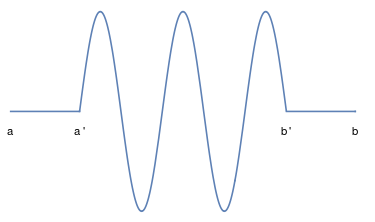
\includegraphics[scale=0.4]{./img/testfuncion.png}
\end{center}

Definimos $\Psi(x)=\integral{a'}{x}{\phi(s)ds}$ y tenemos $\Psi'=\phi$. Falta probar que $\Psi\in\mathcal{D}(a,b)$.
Si $x\leq a'$, claramente $\Psi(x)=0$ \big($\phi(x)=0\quad\forall x\in(a,a')$\big). Si $x\geq b'$,
\[
\int_{a'}^x\phi(s)ds=\int_{a'}^{b'}\phi(s)ds=\int_{a}^{b}\phi(s)ds=0
\]
Por tanto $\supp\Psi\subset[a',b']$.

\end{proof}

\begin{lemma}
\label{lemma:14}
Sea $f\in C(a,b)$ tal que $\integral{a}{b}{f(x)\phi'(x)dx=0}\espacio\forall\phi\in\mathcal{D}(a,b)\Longrightarrow f \text{ es constante.}$
\end{lemma}

\begin{proof}
Sea $x_0\in(a,b)$, tomamos una función $\phi_{x_0}\in \soportecompacto$ cumpliendo la tesis del lema \ref{existenciaphi}. Podemos tomarla de forma que $\integral{a}{b}{\phi_{x_0}(s)ds}=1$ (multiplicándola por cierta constante). 

Definimos $\Psi(x)=\integral{a}{x}{\phi_{x_0}(s)ds}$ y tomamos $c$ de forma que:
\[
\integral{a}{b}{f(s)\Psi'(s)}=c\integral{a}{b}{\Psi'(s)ds}=c\Psi\Big|_a^b=c
\]
Tomamos $\phi\in\soportecompacto$ y veamos que la función $\phi-\lambda\Psi'$ tiene primitiva para cierto $\lambda\in\R$. Supongamos que tiene media 0, y despejemos $\lambda$:
\[
\integral{a}{b}{\phi(s)-\lambda\Psi'(s)}=0 \Longrightarrow \lambda=\integral{a}{b}{\phi(s)ds}
\]
Haciéndo esa elección de $\lambda$, $\phi-\lambda\Psi'$ tiene primitiva por el lema \ref{lemma:13}.
\[
0=\integral{a}{b}{f(s)(\phi(s)-\lambda\Psi'(s))ds}=\integral{a}{b}{f(s)\phi(s)ds}-\lambda\integral{a}{b}{f(s)\Psi'(s)ds}=
\]
\[
=\integral{a}{b}{f(s)\phi(s)ds}-c\integral{a}{b}{\phi(s)ds}=\integral{a}{b}{(f(s)-c)\phi(s)ds} \Rightarrow f(s)-c=0 \Rightarrow f\equiv c
\]
\end{proof}

\begin{lemma}
Sean $f$,$g$ funciones continuas en $(a,b)$, entonces es equivalente:
\[
\integral{a}{b}{g\phi}+\integral{a}{b}{f\phi'}=0 \espacio \forall\phi\in\soportecompacto \Longleftrightarrow f\in C^1(a,b), g=f'
\]
\end{lemma}

\begin{proof}

($\Rightarrow$)Tomamos $x_0\in(a,b)$ y definimos $\tilde{f}(x)=\integral{a}{x}{g(s)ds}\Rightarrow \tilde{f}\in C^1$.
\[
\integral{a}{b}{\tilde{f}(s)\phi'(s)+g(s)\phi(s)ds}=\integral{a}{b}{\tilde{f}(s)\phi'(s)+\tilde{f}'(s)\phi(s)ds}=\integral{a}{b}{(\tilde{f}\phi)}=\tilde{f}\phi\Big|_a^b=0
\]
Restando la expresión de la hipótesis menos la anterior, obtenemos:
\[
0=\integral{a}{b}{f(s)\phi'(s)ds}-\integral{a}{b}{\tilde{f}(s)\phi'(s)ds}=\integral{a}{b}{(f-\tilde{f})(s)\phi'(s)ds}
\]
Y usnado el lema \ref{lemma:14}, tenemos que $f-\tilde{f}$ es constante, luego $f\in C^1$ ya que $\tilde{f}$ también pertenece a $C^1$.

($\Leftarrow$) 
\[
0=f\phi(x)\Big|_a^b=\integral{a}{b}{(f(x)\phi(x))'dx}=\integral{a}{b}{f(x)\phi'(x)dx+f'(x)\phi(x)dx}
\]
\end{proof}

\section{Problema de Braquistocrona}

Este problema se centra principalmente en averiguar que forma (curva) tenemos que darle a un tobogán para que este sea el más rápido.

A esa curva la vamos a denotar por $Y(t)$ y vamos a suponer que  pertenece a $C^1(0,L)$, es decir, que no tenga picos. Además, vamos a suponer que el tobogán tiene altura máximo 1, y mínima 0, es decir, $Y(0)=1$ e $Y(L)=0$. También necesitamos que el tobogán tenga sentido, es decir, que no tenga subidas ni bajadas muy bruscas, luego necesitamos imponer $Y(x)<1 \espacio \forall x \in (0,L)$.

Recordemos primero algunas nociones de física. Vamos a denotar por $(x(t),y(t))$ a la posición de una persona en el tobogán en el instante $t\in[0,T]$, por $m$ a su masa y por $g$ a la gravedad. Recordemos que la expresión de la energía potencial es $mgy(t)$, la de la velocidad es $v(t)=\sqrt{x'(t)^2+y'(t)^2}$ y la de la energía cinética es $\frac{mv(t)^2}{2}$.

Si hacemos el tobogán suficientemente suave, por el teorema de conservación de la energía, se cumple:

\begin{equation}
\label{equationff}
mgy(t)+\frac{m}{2}(x'(t)^2+y'(t)^2)\equiv cte
\end{equation}
En el primer momento nos dejamos caer, luego en $t=0$, $(\ref{equationff})=mg$

Tenemos entonces $y(t)=Y(x(t)) \Rightarrow y'(t)=Y'(x(t))x'(t)$, sustituyendo en (\ref{equationff}):
\[
mgY(x(t))+\frac{m}{2}x'(t)^2+\frac{m}{2}(Y'(x(t))x'(t))^2=mg
\]
\[
x'(t)^2\left(1+Y'(x(t))^2\right)=2g\left(1-Y(x(t))\right)\Rightarrow x'(t)=\sqrt{2g}\sqrt{\frac{1-Y(x(t))}{1+Y'(x(t))^2}}
\]
Estamos buscando el tiempo de llegada, $T$, ¿cómo lo hacemos? Aplicamos un truco típico de ecuaciones diferenciales:
\[
T = \integral{0}{T}{dt}=\integral{0}{T}{\frac{x'(t)}{x'(t)}dt}=
\frac{1}{\sqrt{2g}}\integral{0}{T}{\frac{\sqrt{1+Y'(x(t))^2}}{\sqrt{1-Y(x(t))}}x'(t)dt}
\]
Que tras el cambio de variable $x=x(t)$ nos queda:
\[
T=\frac{1}{\sqrt{2g}}\integral{0}{L}{\frac{\sqrt{1+Y'(x)^2}}{\sqrt{1-Y(x)}}dx}
\]
Definimos ahora el conjunto de funciones donde vamos a buscar nuestro mínimo:
\[
D=\{y\in C^1(0,L),y(0)=1,y(L)=0, y'(x)<1 \espacio \forall x \in(0,L)\}
\]
Y definimos nuestro funcional:
\[
L(y)=\integral{0}{L}{\frac{\sqrt{1+Y'(x)^2}}{\sqrt{1-Y(x)}}dx}
\]
Usando la notación del principio, tenemos una función $F$ tal que $F(x,y,p)=\sqrt{\frac{1+p^2}{1-y}}$

Usando el Teorema \ref{theorem:12} podemos definir:
\[
Z(x)=\derivada{F}{p}(x,y,y')=\frac{1}{\sqrt{1-y(x)}}\frac{y'(x)}{\sqrt{1+y'(x)^2}} \in C^1(0,T)
\]
Ahora, despejando $y'(x)$, vamos a ver que $y\in C^2$. Definiendo $\Psi(y')=\frac{y'}{\sqrt{1+y'^2}}=Z(x)\sqrt{1-y}$. Como $\Psi(s)=\frac{s}{\sqrt{1+s^2}}$ tiene inversa de clase 1, tenemos:
\[
y'(x)=\Psi^{-1}(Z(x)\sqrt{1-y(x)})\Rightarrow y\in C^2
\]
En general, tenemos que si $F$ no depende de $x$, podemos hacer:
\[D(x)=F(y(x),y'(x))-Z(x)y'(x)\Rightarrow D'(x)=
\]
\[=\derivada{F}{y}(y(x),y'(x))y'(x)+\derivada{F}{p}(y(X),y'(x))y''(x)-Z'(x)y'(x)-Z(x)y''(x)=\]
\[
=y'(Z'(x)-Z'(x))=0
\]
Es decir, para alguna constante $C\in\R$, tenemos que:
\[
F(y(x),y'(x))-Z(x)y'=C
\]
En nuestro caso particular, nos quedaría:
\[
\frac{\sqrt{1+y'(x)^2}}{1-y(x)}-\frac{1}{\sqrt{1-y(x)}}\frac{y'(x)^2}{\sqrt{1+y'(x)^2}}=0 \Rightarrow \frac{1}{\sqrt{1-y(x)}}\frac{1}{\sqrt{1+y'(x)^2}}=C
\]
Esa ecuación diferencial, es de variables separadas, deberíamos resolverla con las condiciones iniciales $y(0)=1,y(L)=0$, pero la solución es trascendente, es decir, no tiene expresión explícita, es un cicloide.

\begin{figure}[!ht]
   \center
  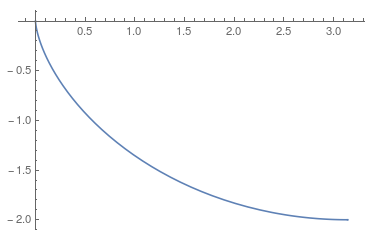
\includegraphics[scale=0.5]{img/cicloide.png}
  \caption{Ejemplo de cicloide}
\end{figure}

\section{Relación de ejercicios}

\begin{ejercicio}
Encontrar la curva en la que el siguiente funcional podría alcanzar su extremo:
\[
I(y)=\integral{1}{2}{\Big(y'(x)^2-2xy(x)\Big)dx}
\]
con condiciones de contorno $y(1)=0,y(2)=-1$.
\end{ejercicio}
\textbf{Solución:}
Definimos $F(x,y,p)=p^2-2xy$ y obtenemos:
\[
\derivada{F}{p}=2p, \espacio \derivada{F}{y}=-2x \Rightarrow Z(x)=2y'(x), \espacio Z'(x)=-2x
\]
Resolviendo la ultima ecuación, obteniendo:
\[
Z(x)=-x^2+C \Rightarrow 2y'(x)=-x^2+C \Rightarrow y'(x)=\frac{-x^2+C}{2}\Rightarrow y(x)=-\frac{x^3}{6}+\frac{c}{2}x+D
\]
Usando las condiciones de contorno, podemos calcular el valor de $C$ y $D$, obteniendo:
\[
y(x)=\frac{x-x^3}{6}
\]
\begin{ejercicio}
Encuentra las curvas que unen $(1,3)$ con $(2,5)$, que puedan ser extremos del funcional:
\[
I(y)=\integral{1}{2}{\Big(y'(x)+x^2y'(x)^2\Big)dx}
\]
\end{ejercicio}

\textbf{Solución} $y(x)=-\frac{4}{x}+7$

\begin{ejercicio}
  Sean $\Phi\in \mathcal{C}^1(\mathbb{R}^3), y(x)\in \mathcal{C}^2\xcero, y'(x) \neq 0$. Dado el funcional
  \[
    F[y] = \int_{a}^{b}{\Phi(x,y(x),y'(x))dx}
  \]
  demuéstrese la equivalencia de las dos formas siguientes de las
  ecuaciones de Euler-Lagrange.
  \begin{itemize}
  \item[$a)$] $\frac{\partial\Phi}{\partial y}-\frac{d}{dx}\frac{\partial\Phi}{\partial p} = 0 $
  \item[$b)$] $\frac{\partial\Phi}{\partial x} - \frac{d}{dx}(\Phi-y'\frac{\partial\Phi}{\partial p}) = 0$
  \end{itemize}
  \begin{proof}
    Comenzamos viendo el caso $a) \implies b)$. Del apartado $a)$ sabemos que
    \[
      \frac{\partial\Phi}{\partial y} = \frac{d}{dx}\frac{\partial\Phi}{\partial p}
    \]
    y del enunciado sabemos que $\Phi$ es de calse $\mathcal{C}^1$
    luego $\frac{\partial\Phi}{\partial p}$ es de $\mathcal{C}^1$.

    Cuando derivamos $\Phi(x,y(x),y'(x))$ obtenemos
    \begin{align*}
      \frac{d\Phi}{dx}(x,y(x),y'(x)) & = \frac{\partial\Phi}{\partial x}(x, y(x), y'(x)) \\
                          & + \frac{\partial\Phi}{\partial y}(x, y(x), y'(x))y'(x) \\
                          & + \frac{\partial\Phi}{\partial p}(x, y(x), y'(x))y''(x)
    \end{align*}
    Recordemos que $\frac{\partial\Phi}{\partial p}(x, y(x), y'(x)) = z(x)$ luego
    \begin{align*}
      \frac{d}{dx}(\Phi-y'\frac{\partial\Phi}{\partial p}) & = \Phi_x + \Phi_yy' + \Phi_py'' - y''z -y'z'
    \end{align*}
    Tenemos que el 3º y 4º termino son opuestos, al igual que el 2º y 5º, luego obtenemos
        \begin{align*}
      \frac{d}{dx}(\Phi-y'\frac{\partial\Phi}{\partial p}) = \Phi_x
        \end{align*}

        que es lo que queríamos.

        $b)\implies a)$
        
        Todos los pasos que hemos dado son reversibles pero
        necesitamos ver que
        $\frac{\partial\Phi}{\partial p}(x, y(x), y'(x))$ es $\mathcal{C}^1$.

        Llamando $H(x) = \Phi-y'(x)z(x)$, por hipótesis tenemos que
        $H$ es derivable. Despejando tenemos que

        \[
          z = \frac{\Phi-H}{y'}
        \]

        luego $z$ es derivable por ser cociente de derivables ($y'\neq 0$).

        \begin{align*}
          \Phi_x & = \Phi_x + \Phi_yy' + \Phi_py'' - y''z -y'z' \\
                 & \implies y'(\Phi_y-z') = 0
        \end{align*}

        e $y' \neq 0$ por hipótesis, luego $\Phi_y - z' = 0$.
  \end{proof}
\end{ejercicio}
\begin{ejercicio}
Obténgase la forma que adopta la ecuación de Euler-Lagrange en los siguientes casos particulares:

\begin{enumerate}[a)]
\item $\Phi$ sólo depende de $y'$.
    \begin{proof}
      Usando el apartado a) del ejercicio anterior y sustituyendo $\frac{\partial\Phi}{\partial y}=0$ obtenemos
      \[
        \frac{d}{dx}\Phi_p = 0
      \]

      De donde deducimos que $\Phi_p(y'(x))$ es una constante.
    \end{proof}
\item $\Phi$ no depende de $y$.
\item $\Phi$ no depende explícitamente de $x$.
\item $\Phi=G(x,y)\sqrt{1+y'^2}$.
\end{enumerate}
\end{ejercicio}

\begin{ejercicio}
Aplíquense los resultados anteriores a los ejemplos siguientes:
\begin{enumerate}[a)]
\item $\mathcal{F}(y(x))=\integral{}{}{y(2x-y)dx}$, $y(0)=0$, $y(\pi/2)=\pi/2$.
\item $\mathcal{F}[y(x)] =\integral{}{}{y(2x-y)dx}, \quad y(0) = 0, \quad y(\pi/2) = \pi/2$

    Definimos $F(x,y,p) = y(2x-y)$. Se cumple

    \begin{align*}
      F_p &= 0\\
      z(x) &= 0\\
      F_y(x,y(x)) &= 2y(x)-2x
    \end{align*}

    De aquí obtenemos $2x-2y = 0 \implies y(x) = x$. Ahora tenemos que
    comprobar que la solución cumple las condiciones de contorno.

    \[
      y(0) = 0, \quad y(\pi/2) = \pi/2
    \]
    
    Luego se cumplen ambas condiciones.
\item $\mathcal{F}(y(x))=\integral{}{}{(y^2+2xyy')dx}$, $y(a)=A$, $y(b)=B$.
\item $\mathcal{F}(y(x))=\integral{}{}{y'(1+x^2y')dx}$, $y(1)=3$, $y(2)=5$.
\end{enumerate}
\end{ejercicio}



\chapter{Derivadas débiles}

Recordemos el espacio $L^1(a,b)$ de las funciones $\funcion{f}{(a,b)}{\R}$ que son Lebesgue integrables. Ese espacio estaba formado por clases de equivalencia, que normalmente llamamos clases de funciones. Que sea Lebesgue integrable, no quiere decir que sea continua, como nos indica la \textit{función de Dirichlet}, que es Lebesgue integrable pero evidentemente no es continua.
\[
f(x)=\left\{
\begin{array}{cc}
0 & x\notin\mathbb{Q} \\
1 & x\in\mathbb{Q}
\end{array}
\right. 
\]
Toda función continua no es integrable, necesitamos que esté acotada. Eso nos dice que todas las funciones continuas no están en $L^1(a,b)$. Para evitar eso, definimos el \textit{espacio de funciones continuas localmente integrables}, que denotaremos por:
\[
L^1_{loc}(a,b)=\{\funcion{f}{(a,b)}{\R} \;|\; \forall J \text{ intervalo compacto},f_{|J}\text{ es integrable}\}
\]
Ese espacio soluciona el problema anterior ya que todas las funciones continuas sí son localmente integrables. Solucionado el problema, podemos definir la derivada débil con tranquilidad:

\begin{definition}
Sean $f,g\in\localmenteintegrable$, se dice que $g$ es la derivada débil de $f$ si se verifica que:
\[
\integral{a}{b}{f\phi'}+\integral{a}{b}{g\phi}=0 \espacio \forall\phi\in\soportecompacto
\]
\end{definition}

Cabe resaltar, que la definición anterior implica que la derivada débil de una función no es única, es decir, una función $f$ puede admitir varias derivadas débiles. Sin embargo, como veremos en el siguiente corolario, serán iguales para casi todo punto.

\section{Propiedades básicas}

Podemos generalizar el lema fundamental del cálculo de variciones:

\begin{theorem}
Si $f\in\localmenteintegrable$ cumpliendo:
\[
\integral{a}{b}{f(x)\phi(x)dx}=0 \espacio\forall\phi\in\soportecompacto
\]
Entonces $f(x)=0$ $a.e$ $x\in(a,b)$.
\end{theorem}
Este resultado engloba al visto previamente en el teorema \ref{theorem:1.3}. Como consecuencia, tenemos:
\begin{coro}
Sea $f\in\localmenteintegrable$ y $g,\tilde{g}\in\localmenteintegrable$ dos derivadas débiles de $f$. Entonces $g(x)=\tilde{g}(x)$ $a.e$ $x\in(a,b)$.
\end{coro}

\begin{proof}
Simplemente usando la definición y el lema generalizado tenemos:
\[
\left.
\begin{array}{c}
\integral{a}{b}{f\phi'}+\integral{a}{b}{g\phi}=0 \\
\integral{a}{b}{f\phi'}+\integral{a}{b}{\tilde{g}\phi}=0
\end{array}
\right\} \Rightarrow \integral{a}{b}{(g-\tilde{g})\phi}=0 \Rightarrow g=\tilde{g} \; a.e
\]
\end{proof}

Para la demostración del lema generalizado, necesitaremos algunas herramientos previas. Recordemos primeramente una propiedad de las funciones Lebesgue integrables:

\begin{prop}
Dado $f\in\localmenteintegrable$, existe una secuencia de funciones simples, $\{g_n\}$, tal que $\{g_n\}\longrightarrow f$.
\end{prop}

\begin{lemma}
Sea $g$ una función simple, entonces existe una sucesión de funciones de soporte compacto $\phi_n\in\soportecompacto$ tal que $\{\phi_n\}\longrightarrow g \; a.e$ y además $|\phi_n(x)|\leq|g(x)|$.
\end{lemma}

Ahora ya sí podemos demostrar el lema generalizado:

\begin{proof}
Sea $g$ una función simple. Por el lema anterior, puedo tomar una sucesión $\phi_n$ de funciones de soporte compacto convergiendo a $g$.Usando el teorema de la convergencia dominada de Lebesgue, podemos intercambiar el límite en la siguiente integral:
\[
\limitemasinfinito{n}{\integral{}{}{\phi_n(x)f(x)dx}}=\integral{}{}{g(x)f(x)}dx
\]
Por la proposición anterior, nos podemos tomar una sucesión $g_n$ de funciones simples de forma que $\{g_n\}\longrightarrow f \; a.e$. De forma análoga:
\[
0=\limitemasinfinito{n}{\integral{}{}{g_n(x)f(x)dx}}=\integral{}{}{f(x)^2}dx \Rightarrow f\equiv 0 \; a.e
\]
\end{proof}

La derivada débil tiene una propiedad parecida a la derivada clásica, ambas son conceptos locales, es decir:

\begin{prop}
Si $f$ es una función que admite derivada débil $f'=g$ en $(a,b)$, y tomamos $(a',b')\subset(a,b)$, entonces $f_{|(a',b')}$ admite derivada débil y vale $g_{|(a',b')}$.
\end{prop}

\begin{proof}
Evidente usando el hecho de que $\mathcal{D}(a',b')\hookrightarrow\soportecompacto$.
\end{proof}

Toda función derivable no es derivable débil, como ilustra el siguiente ejemplo:

\begin{example}
La función $\funcion{f}{\R}{\R}$ definida por $f(x)=\sqrt{|x|}$, es derivable débil pero no derivable.

Primero tenemos que ver que $g\in\localmenteintegrable$. Si el intervalo compacto $J$ escogido no contiene al 0, entonces podemos integral sin problema. En caso contrario, tenemos que ver qué pasa con la siguiente integral:
\[
\integral{-\varepsilon}{\varepsilon}{|g(x)|dx}\overset{g\; simetrica}{=}2\integral{0}{\varepsilon}{|g(x)|dx}=2\integral{0}{\varepsilon}{\frac{1}{2\sqrt{x}}}=2\sqrt{x}\Big|_0^\varepsilon=2\sqrt{\varepsilon}<+\infty
\]
Ahora tenemos que comprobar que $g$ es la derivada débil de $f$, es decir:
\[
\integral{\R}{}{f\phi'}+\integral{\R}{}{g\phi}=0 \espacio \forall\phi\in\soportecompacto
\]
\[
\integral{\R}{}{f(x)\phi'(x)dx}=\integral{|x|>\varepsilon}{}{f(x)\phi'(x)dx}+\underbrace{\integral{|x|<\varepsilon}{}{f(x)\phi'(x)dx}}_{f\phi'\leq2\sqrt{\varepsilon}\max\phi'\to0}=\integral{|x|>\varepsilon}{}{f(x)\phi'(x)dx}=
\]
\[
=\integral{-\infty}{-\varepsilon}{f(x)\phi'(x)dx}+\integral{\varepsilon}{+\infty}{f(x)\phi'(x)dx}=
\]
\[
=\underbrace{f(x)\phi(x)\Big|_{-\infty}^{-\varepsilon}}_{=f(-\varepsilon)\phi(-\varepsilon)\to 0}-
\integral{-\infty}{-\varepsilon}{g(x)\phi(x) dx}+
\underbrace{f\phi\Big|_{\varepsilon}^{+\infty}}_{{=f(\varepsilon)\phi(\varepsilon)\to 0}}-
\integral{\varepsilon}{+\infty}{g(x)\phi(x) dx}=
\]
\[
-\integral{\R}{}{g(x)\phi(x)dx}+\underbrace{\integral{|x|<\varepsilon}{}{g(x)\phi(x)dx}}_{\to0}=-\integral{\R}{}{g(x)\phi(x)dx}
\]
\end{example}

Vamos a ver que la derivada de una integral de una derivada débil, es la propia función (como es de esperar). Para ello vamos a tener que desarrollar una serie de pasos previos.

\begin{theorem}
\label{fundamentalcalculo}
Sea $g\in\localmenteintegrable$ y tomo $x_0\in(a,b)$. Defino $\funcion{f}{(a,b)}{\R}$ como
\[
f(x)=\integral{x_0}{x}{g(x)ds}
\]
Entonces $f'=g$ y $f\in C[a,b]$.
\end{theorem}

\begin{proof}

La integral en $f$ tiene sentido ya que $[x_0,x]\subset (a,b)$. Comprobemos que $f\in C(a,b)$. Tomamos $\{x_n\}$ sucesión de puntos de $(x_0,x)$ tal que $x_n\to \tilde{x}\in[x_0,x]$ (por ser compacto).

\begin{center}

\begin{tikzpicture}[scale=0.5]
\draw (-1,0)-- (9,0); %Axis

\draw (0,-.5) -- (0,.5);
\draw (0,-0.5) node[anchor=north] {$a$};

\draw [thick] (2.1,-.5) -- (2,-.5) -- (2,.5) -- (2.1,.5); 
\draw (2,-.5) node [anchor=north] {$x_0$};

\draw (3.5,-.5) -- (3.5,.5);
\draw (3.5,-0.5) node[anchor=north] {$x_n$};

\draw (4.5,-.5) -- (4.5,.5);
\draw (4.5,-0.5) node[anchor=north] {$\tilde{x}$};

\draw [thick] (6,-.5) -- (6.1,-.5) -- (6.1,.5) -- (6,.5); 
\draw (6,-.5) node [anchor=north] {$x$};

\draw (8,-.5) -- (8,.5);
\draw (8,-0.5) node[anchor=north] {$b$};

\end{tikzpicture}
\end{center}

\begin{enumerate}[-]
\item Si $x\notin[x_0,\tilde{x}] \Rightarrow x\notin [x_0,x_n]$ para $n\geq n_0$.
\item Si $x\in(x_0,\tilde{x}) \Rightarrow x\in [x_0,x_n]$ para $n\geq n_0$.
\end{enumerate}

Y ese es la clave que nos va a permitir ver que $f(x_n)\to f(\tilde{x})$. Sea $J$ un intervalo compacto de forma que $[x_0,x]\subset J\subset(a,b)$.
\[
\integral{x_0}{x_n}{g(x)dx}=\integral{J}{}{g(x)\chi_{[x_0,x_n]}}(x)dx
\]
Usando lo anterior obtenemos la convergencia puntual de la sucesión $g(x)\chi_{[x_0,x_n]}\overset{cp}{\longrightarrow}g(x)\chi_{(x_0,\tilde{x})}$. Lo que nos da la convergencia en integral también:
\[
f(x_n)=\integral{J}{}{g(x)\chi_{[x_0,x_n]}(x)dx}\overset{cp}{\longrightarrow}\integral{J}{}{g(x)\chi_{(x_0,\tilde{x})}(x)dx}=\integral{x_0}{\tilde{x}}{g(x)dx}=f(\tilde{x})
\]
Luego $f\in C(a,b) \Rightarrow f\in \localmenteintegrable$.
Ahora nos queda ver $f'=g$. Para ello tenemos que comprobar que:
\[
\integral{a}{b}{f(x)\phi'(x)dx}+\integral{a}{b}{g(x)\phi(x)dx}=0 \espacio \forall \phi\in \soportecompacto
\]
Tenemos el problema de que $g$ no tiene por qué ser derivable (podría ser una función escalón, por ejemplo). Vamos a empezar suponiendo que $g\in L^1([a,b])$ (para que $f$ esté bien definida) y que $x_0=a$. Al final reduciremos esas hipótesis hasta llegar a que $g\in\localmenteintegrable$.

\underline{Paso 1}: $g\in L^1([a,b])$ y $x_0=a$. Para ver que
\[
\integral{a}{b}{f(x)\phi'(x)dx}=-\integral{a}{b}{g(x)\phi(x)dx} 
\]
vamos a tener que usar el Teorema de Fubini-Tonelli.
\[
\integral{a}{b}{f(x)\phi'(x)dx}=
\integral{a}{b}{\left(\integral{a}{x}{g(s)ds}\right)\phi'(x)dx}\overset{TªFT}{=}
\integral{a}{b}{\left(\integral{s}{b}{g(s)\phi'(x)dx}\right)ds}=\]
\[
\integral{a}{b}{g(s)\left(\integral{s}{b}{\phi'(x)dx}\right)ds}
=\integral{a}{b}{g(s)(\underbrace{\phi(b)}_{=0}-\phi(s))ds}=-\integral{a}{b}{g(s)\phi'(s)ds}
\]
\underline{Paso 2}: Reemplazamos la hipótesis $x_0=a$ por $x_0\in(a,b)$ y usamos el paso 1:
\[
\integral{a}{b}{g(x)\phi(x)dx}=-\integral{a}{b}{\left(\integral{a}{x}{g(s)ds}\right)\phi'(x)dx}
\]
Vemos que la integral del interior se puede expresar como una constante más una función:
\[
\integral{a}{x}{g(s)ds}=\underbrace{\integral{a}{x_0}{g(s)ds}}_{cte=C}+\underbrace{\integral{x_0}{x}{g(s)ds}}_{funcion}
\]
Luego:
\[
-\integral{a}{b}{\left(\integral{a}{x}{g(s)ds}\right)\phi'(x)dx}=
-\underbrace{\integral{a}{b}{B\phi'(x)dx}}_{=B(\phi(b)-\phi(a))=0}-\integral{a}{b}{\left(\integral{x_0}{x}{g(s)ds}\right)\phi'(x)dx}=
-\integral{a}{b}{f(x)\phi(x)dx}
\]
\underline{Paso 3}: Ahora sustituimos la hipótesis $g\in L^1([a,b])$ por $g\in\localmenteintegrable$. Tomamos un subintervalo compacto $[a'.b']\subset(a,b)$ donde $g_{|[a'.b']}\in L^1([a',b'])$, de forma que $\supp\phi\subset[a',b']$. Sea $x_0\in[a',b']$ y $x\in(a,b)$.

Ahora aplicamos el caso 2, usando que $\supp\phi\subset[a',b']$:
\[
\integral{a}{b}{g(x)\phi(x)dx}=\integral{a'}{b'}{g(x)\phi(x)dx}=-\integral{a'}{b'}{\left(\integral{x_0}{x}{g(s)ds}\right)\phi'(x)dx}=-\integral{a}{b}{f(x)\phi'(x)dx}
\]
\end{proof}

Una vez obtenida una versión para derivadas débiles del Teorema Fundamental del Cálculo, vamos a ver más propiedades de este concepto.

La siguiente proposición nos permitirá obtener un representante continuo a partir de una función que tenga derivada débil, pero no tengo por qué ser continua.

\begin{prop}
\label{representantecontinuo}
Si $f\in\localmenteintegrable$ tiene derivada débil en $(a,b)$, entonces existe $\tilde{f}\in C(a,b)$ tal que $\tilde{f}(x)=f(x)$ $a.e$ $x\in(a,b)$.
\end{prop}

\begin{proof}
Sea $f\in\localmenteintegrable$, $\funcion{g}{(a,b)}{\R}$ su derivda débil, es decir, $f'=g$ y $x_0\in(a,b)$. Definimos $\funcion{\tilde{f}}{(a,b)}{\R}$ por:
\[
\tilde{f}(x)=\integral{x_0}{x}{g(s)ds}
\]
El resultado anterior nos da que $\tilde{f}\in C(a,b)$ y $\tilde{f}'=g$. Solo nos falta ver que $\tilde{f}$ es igual casi por doquier a $f$, o lo que es lo mismo, comprobar que $f-\tilde{f}$ tiene derivada débil 0:
\[
\left.
\begin{array}{cc}
\integral{a}{b}{f(x)\phi'(x)dx}=-\integral{a}{b}{g(x)dx} \\
\integral{a}{b}{\tilde{f}(x)\phi'(x)dx}=-\integral{a}{b}{g(x)dx}
\end{array}
\right\} \Rightarrow \integral{a}{b}{(f-\tilde{f})(x)\phi'(x)}=-\integral{a}{b}{0\phi(x)dx}
\]
\end{proof}

\begin{prop}
\label{derivadadebilcero}
Si $f\in\localmenteintegrable$ y tiene derivada débil igual a 0, entonces $f$ es constante $\casipordoquier$.
\end{prop}

\begin{proof}
La demostración de este es prácticamente igual a la demostración del Lema \ref{lemma:14}.
\end{proof}

\begin{example}[examen 18/19]
Sea $\funcion{f}{\R\backslash\{1\}}{\R}$ definida por $f(x)=\frac{(x-1)(x+2)}{|x-1|}$. ¿Tiene derivada débil?

Nos damos cuenta de que $f(x)=\frac{(x-1)(x+2)}{|x-1|}=\frac{x-1}{|x-1}(x+2)$, es decir, $f$ se expresa como producto de una función escalón (discontinua), por un polinomio (continuo), luego $f$ es discontinua.

Como es discontinua, si tuviera derivada débil, por la proposición \ref{representantecontinuo} , debe existir $\tilde{f}$ función continua tal que $f(x)=\tilde{f}(x)\;\; a.e$. Veamos que esa función no puede existir. El conjunto $\{x:\;\; f(x)=\tilde{f}(x)\}$ tiene \textbf{medida llena} (complementario con medida nula), luego es denso. Tomamos $\{x_n\}\longrightarrow 1$ y vemos que:
\[
3=\limite{n}{1^+}{f(x_n)}=\limite{n}{1^+}{\tilde{f}(x_n)}
\]
\[
-3=\limite{n}{1^-}{f(x_n)}=\limite{n}{1^-}{\tilde{f}(x_n)}
\]
Pero $\tilde{f}$ es continua, luego esos límites deberían coincidir: contradicción.

\end{example}

\begin{prop}
\label{derivadanesima}
Sea $f\in\localmenteintegrable$ $n$-veces derivable débil, entonces existe $\tilde{f}$ tal que $f(x)=\tilde{f}(x) \; \casipordoquier$ y además $\tilde{f}\in C^{n-1}(a,b)$.
\end{prop}

\begin{proof}
\underline{Caso n=1}: Si $f$ tiene derivada débil, sabemos por la proposición \ref{representantecontinuo} que existe $\tilde{f}\in C(a,b)$ y $f(x)=\tilde{f}(x) \;\casipordoquier$.
El caso $n$ se deduce fácilmente del siguiente hecho:
\[
\left.
\begin{array}{r}
\integral{a}{b}{\tilde{f}(x)\phi'(x)dx}+\integral{a}{b}{g(x)\phi(x)dx}=0 \\
\tilde{f}, g \text{ continuas }
\end{array}
\right\} \Rightarrow \tilde{f}\in C^1(a,b), \;\tilde{f}'=g \text{ (en sentido clásico)}
\]
\underline{Caso n}: Suponemos que $f$ es $(n-1)$-veces derivable débil y que existe $\tilde{f}\in C^{n-2}(a,b)$ tal que $f(x)=\tilde{f}(x)\;\casipordoquier$.
Si derivamos $(n-1)$-veces $f$, obtenemos $\tilde{f}^{n-1)}=f^{n-1)}=g$, que no sabemos si es continua, pero sabemos que podemos elegir un representante que si lo sea. Usando el hecho anterior, tenemos que $\tilde{f}\in C^{n-1}(a,b)$.
\end{proof}

\section{The Devil Staircase}

Nuestro objetivo va a ser construir una función continua$\funcion{f}{\R}{\R}$ que no admita derivada débil.

En $\R\backslash(0,1)$ será constante:
\[
f(x)=\left\{
\begin{array}{cc}
0 & x\leq 0\\
1 & x\geq 1
\end{array}
\right.
\]
En $(0,1)$ nos va a costar un poco más construirla. Para ello, definimos primeramente \textit{el conjunto ternario de Cantor}, que se construye sobre el intervalo $[0,1]$, eliminando en cada paso el segmento abierto correspondiente al tercio central de cada intervalo.

\begin{figure}[h]
   \center
  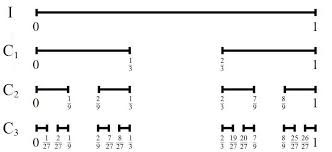
\includegraphics[scale=0.5]{img/cantor.jpeg}
  \caption{Representación gráfica}
\end{figure}

Es fácil ver que la media del primer conjunto $C_0$ es $2/3$, el de $C_1$ $4/9$, y el de $C_n=(\frac{2}{3})^n$. Además, cada $C_n$ es compacto, luego si consideramos como conjunto $C$ a la intersección de todos, es decir, $C=\cap_{n\in\N} C_n$, obtenemos otro conjunto compacto. $C$ tiene media nula, ya que $\mu(C)=\left(\frac{2}{3}\right)^n\to0$.

Vamos a construir nuestra $f$ sobre el complementario de ese conjunto, es decir, sobre $B=(0,1)\backslash C$.

Nuestra función será constante en cada intervalo de $B$, es decir, en los intervalos que hemos sustraído al construir el conjunto ternario de Cantor. Para hacerla continua, necesitamos regularizar cada salto entre intervalos, definiendo $f$ en esa parte como una recta que conecte cada intervalo con el siguiente.

\begin{figure}[H]
   \center
  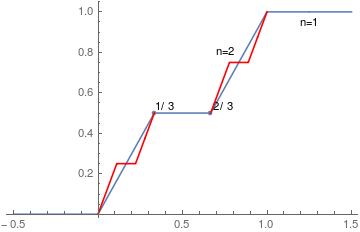
\includegraphics[scale=0.6]{img/escalera.png}
\end{figure}

Denotamos por $f_n$ a la función resultante de realizar el paso anterior $n$ veces, consiguiéndo así una sucesión de funciones continuas. Esta sucesión cumple además una propiedad clave para nosotros: si $x\in B$, existe un $n_0\in\N$ tal que si $n\geq n_0$, entonces $x$, debe de estar en algún intervalo, $I_{n_0}$. Pero en esos intervalos, que son los eliminados por el conjunto de Cantor, nuestra función es constante, es decir, $f_n$ es constante en $I_{n_0}$.

Una vez realiza esta construcción, podemos definir nuestra función $f$ como sigue:
\[
f(x)=\limitemasinfinito{n}{f_n(x)}
\]
Tenemos que ver que $f_n$ converge para que la definición de $f$ tenga sentido. Debido a la forma en la que hemos construido la sucesión $f_n$, tenemos que:

\begin{figure}[H]
   \center
  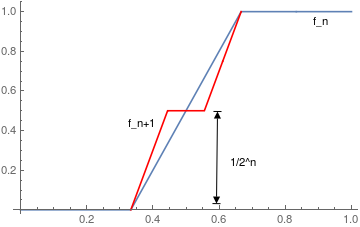
\includegraphics[scale=0.6]{img/convergenciaescalera.png}
\end{figure}
\[
\valorabsoluto{f_n(x)-f_{n+1}(x)}\leq\frac{1}{2^n} \Rightarrow \norm{f_n(x)-f_{n+1}}_{\infty}\leq \frac{1}{2^n}
\]

Expresando ahora $f_n$ usando la forma telescópica de una sucesión:
\[
f_n(x)=f_1(x)+f_2(x)-f_1(x)+...=f_1(x)+\sum_{n=1}^\infty\left(f_{n+1}(x)-f_n(x)\right) \Rightarrow \norm{f_n}_{\infty}\leq \frac{1}{2^n}
\]
Obteniendo así que $f_n$ converge uniformemente a $f$, y como $f_n$ es continua para todo $n\in\N$, $f$ también lo es. 

Ya tenemos nuestra \textit{escalera continua} construida, falta ver que no tiene derivada débil. Supongamos que existe $g$ tal que $f'=g$. Como $f$ está definida como una función constante en cada componente conexa de $B$, su derivada vale 0, es decir, $g(x)=0\;$ si $x \in B$ o $x\leq 1$ o $x\leq 0$. Pero, como $B$ tiene medida llena, lo anterior implica que $g(x)=0 \; a.e \; x\in\R$, luego $f$ sería constante, lo cual es una evidente contradicción.


\end{document}
